\documentclass[12pt, a4paper, oneside]{ctexbook}
\usepackage{amsmath, amsthm, amssymb, bm, graphicx, hyperref, mathrsfs, mhchem, geometry, parskip, siunitx}
\geometry{left = 3.7cm, right = 3.2cm, top = 3cm, bottom = 3cm}

\title{{\Huge{\textbf{基础化学}}}\\笔记}
\author{F1}
\date{\today}
\linespread{1.5}
\newtheorem{theorem}{定理}[section]
\newtheorem{definition}[theorem]{定义}
\newtheorem{lemma}[theorem]{引理}
\newtheorem{corollary}[theorem]{推论}
\newtheorem{example}[theorem]{例}
\newtheorem{proposition}[theorem]{命题}
\newcommand{\ml}{\si{\milli\liter}}
\newcommand{\li}{\si{\liter}}

\begin{document}

\maketitle

\pagenumbering{roman}
\setcounter{page}{1}

%\begin{center}
%    \Huge\textbf{前言}
%\end{center}~\

%这是笔记的前言部分. 
%~\\
%\begin{flushright}
%    \begin{tabular}{c}
%        Dylaaan\\
%        \today
%    \end{tabular}
%\end{flushright}

%\newpage
\pagenumbering{Roman}
\setcounter{page}{1}
\tableofcontents
\newpage
\setcounter{page}{1}
\pagenumbering{arabic}

\chapter{准备知识}
\begin{enumerate}
    \item 特别关注稀溶液(溶液是一个复杂体系);
    \item 关注平衡常数:各种离子间浓度相互制衡;
    \item 关注化学反应的动态, 任意时刻和平衡两个状态;
    \item 体系中温度、压力等条件是变化的, 关注标准态;
    \item 基础化学是重要的工具(理论与实践).
\end{enumerate}

\section*{有效数字}
有效数字是从第一个不为零的数字算起的所有数字. 
\begin{example}
    0.06050为\textbf{四位}有效数字
\end{example}
单位变换不能影响有效数字位数. 
\begin{example}
    10.00 \ml  $\to$ 0.001000 \li 均为四位有效数字
\end{example}


注意: 对于对数数值, 如pH = 11.\textbf{20} 表示 [\ce{H+}]=\textbf{6.3} $\times$ 10$^{-12}$, 为\textbf{两位}有效数字. 
\begin{enumerate}
    \item 其有效数字的位数取决于小数部分的位数
    \item 整数部分只代表该数的方次
\end{enumerate}


\subsubsection{有效数字的意义}
既能表达数值大小, 又能表明测量值准确程度的数字的表示方法, 
它包括测得的全部准确数字和一位可疑数字, 可疑数字的误差内为$\pm$ 1. 刻度型仪器的测量值, 最后一位数字是估计的, 因此是可疑数字. 
\subsubsection{有效数字的修约规则}
\begin{enumerate}
    \item 四舍六入五成双(后面一位数字为5时)5前奇数进位, 偶数舍去. \\例: 1.15 $\to$ 1.2, 1.25 $\to$ 1.2
    \item 若5后有非零数字, 则5进位. \\例: 1.151 $\to$ 1.2
    \item 对原始数据只能进行一次修约, 不能多次修约.
\end{enumerate}

\subsubsection{有效数字的运算法则}
\textbf{只对最后结果进行修约. }
\begin{enumerate}
    \item 加减法: 以小数点后位数最少的数为准. \\例: 50.1 + 1.45 + 0.5812 = \textbf{52.1}
    \item 乘除法: 以有效数字位数最少的数字为准. \\例: 0.0121 $\times$ 25.64 $\times$ 1.05782 = 0.32818231 = \textbf{0.328}
    \item 加减乘除混合运算\\例: 3.489 $\times$ (5.67 - 2.3) = 3.489 $\times$ 3.37(先不修约) \\= 11.75793 = 11.758 = \textbf{12}
    \\例: 6.78 $\times$ 5.903 $\times$ (5.489 - 5.01) = 6.78 $\times$ 5.903 $\times$ 0.479 = 19.1707 = \textbf{19}\\
\end{enumerate}

\subsection*{小结}
\begin{enumerate}
    \item 有效数字的意义: 注意对数与幂形式的转化(pH与浓度)
    \item 有效数字的修约: 4舍6入5成双
    \item 有效数字的运算: 加减 : 看绝对误差最大的,小数点后最少 的
    乘除:看相对误差最大的,有效数字最少的
    
\end{enumerate}

\textbf{只对最后结果进行修约}



\section*{混合物的组成标度}
\begin{enumerate}
    \item 质量分数$w$ \\某溶质质量与混合物质量之比: $w = \frac{m_s}{m}$
    \item 体积分数$\varphi$\\在某一温度下, 溶质体积与混合物体积之比: $\varphi = \frac{V_s}{V}$
    \item 摩尔分数$x$ 某溶质
    \item 质量浓度$\rho $
    \item 物质的量浓度$c$(与温度有关)\\溶液中溶质B的物质的量$n_B$与溶液体积之比: $c_B = \dfrac{\text{溶质B的物质的量(mol)}}{\text{溶液的体积}}$\\
            单位 mol$\cdot$m$^{-3}$, mol$\cdot$L$^{-1}$.\\
            注: 使用$c_B$必须指明基本单元, 对于具体物质, 应将基本单元表示在括号内如$c_{\text{NaCl}}$, 对于溶液, 应将溶剂表示在括号内如$c_{\text{(Ca$^{2+}$)}} = 2$mmol$\cdot$L$^{-1}$
    \item 质量摩尔浓度$b$ (与温度无关)\\单位 mol$\cdot$ kg$^{-1}$\\
            溶液中溶质B的物质的量$n_B$与溶液质量之比: $b_B = \dfrac{\text{溶质B的质量(kg)}}{\text{溶液的质量(kg)}}$\\
\end{enumerate}
例题: 将7.00g草酸晶体()溶解于93.0g水中, 求草酸的摩尔质量浓度$b(\ce{H2SO4})$和摩尔分数$x$.\\

\chapter{稀溶液的依数性}
背景内容
\begin{enumerate}
    \item 溶液的蒸汽压
    \item 溶液的沸点、凝固点
    \item 溶液的渗透压力
\end{enumerate}
\newpage
\section{溶液的基本问题}
温度与压力共同决定物质的形态. \\
\begin{figure}[htbp]
    \centering
    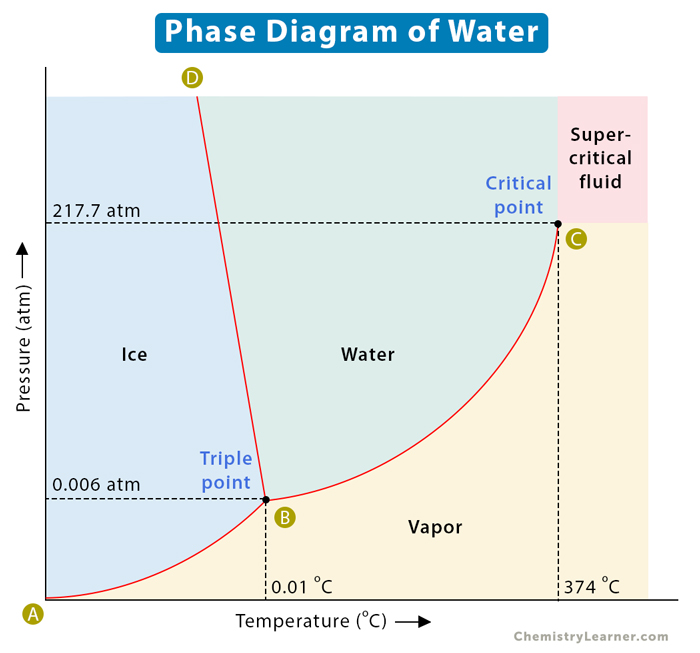
\includegraphics[width=0.8\textwidth]{pics/phase_diagram.jpg}
    \caption{水的相图}
\end{figure}
\subsection{气液平衡: 液体的蒸发、蒸汽压}
\subsubsection{蒸发}
液体从周围环境中吸收热量, 分子动能增加, 部分表层分子克服分子间引力, 逃逸出液面, 形成气体. \\
\subsubsection{凝结}
密闭容器中, 随着蒸发的进行, 由液面溢出的蒸气分子在相互碰撞过程中, 部分分子返回液相, 这个过程叫凝结. \\
\subsubsection{饱和蒸气压}
一定温度下, 密闭容器中, 当液体蒸发与凝结达到动态平衡时, 液体表面上的蒸气与液体之间的相互转化达到平衡. 此时蒸汽压不再增大, 为一定值, 叫做饱和蒸气压, 简称蒸汽压($p$). \\
\subsubsection*{蒸汽压与液体的本性和温度密切相关}
一定温度下, 液体的蒸汽压是一个定值, 与气体的体积、液相的量无关, 只与液体的本性和温度密切有关. 
\begin{figure}[htbp]
    \centering
    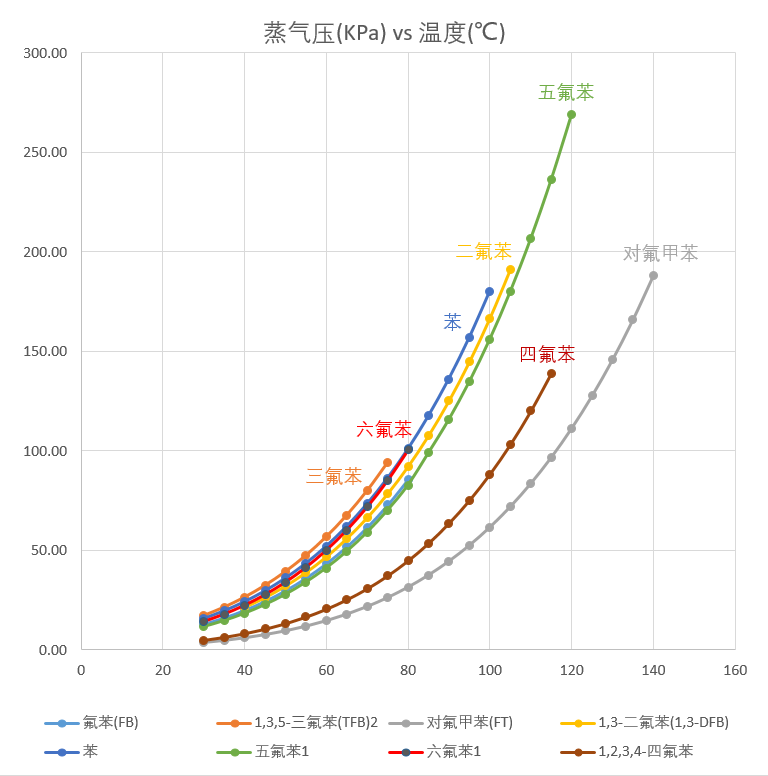
\includegraphics[width=0.8\textwidth]{pics/vapor_pressure.png}
    \caption{蒸汽压-温度曲线}
\end{figure}

\newpage
\subsubsection{液体的沸腾与沸点}
在敞开体系, 升高温度, 液体内部会形成气泡, 当气泡的饱和蒸气压等于外部施予的压强时, 液体内部的气泡就长大并上升, 液体就会沸腾. \\
\subsubsection{液固平衡: 液体的凝固、固体的熔化}
凝固点: 在一定压强下, 液体凝固成固体的温度. \\
从相图来看, 在一定压力下, 物质的液相和固相蒸汽压相等、两相平衡共存的温度, 就是凝固点, 用$T_f$ (freezing point)表示. \\

\subsubsection{蒸汽压的注意要点}
\begin{enumerate}
    \item 液体的蒸汽压与温度有关, 与液体的量无关. 
    \item 蒸汽压与外界大气压相等时, 液体沸腾. 
    \item 蒸汽压大的称为挥发性液体, 蒸汽压小的称为不挥发性液体. 
    \item 
\end{enumerate}


溶液: 两种或两种以上的物质混合在一起, 形成的均匀稳定分散的体系. 
\begin{table}[htbp]
    \centering
    \begin{tabular}{|c|c|c|}
        \hline
         分类方法 & 1 & 2\\
        \hline
        溶质 & 电解质溶液 & 非电解质溶液\\
        \hline
        浓度 & 浓溶液 & 稀溶液\\
        \hline
    \end{tabular}
\end{table}
\\从最简单的体系入手: 难挥发、非电解质、稀溶液



\end{document}